% AquaDiag: 面向低资源水产的多模态诊断对话基准
% 基于 CVPR 2026 模板（中文版）

\documentclass[10pt,twocolumn,letterpaper]{article}

%%%%%%%%% Chinese support
\usepackage[UTF8,fontset=fandol]{ctex}

%%%%%%%%% PAPER TYPE
% \usepackage{cvpr}              % Camera-ready version
\usepackage[review]{cvpr}        % Review version
% \usepackage[pagenumbers]{cvpr} % Force page numbers

% Import additional packages in the preamble file, before hyperref
%% Additional preamble for AquaDiag paper.

%% Inline annotations
\newcommand{\red}[1]{{\color{red}#1}}
\newcommand{\todo}[1]{{\color{red}#1}}
\newcommand{\TODO}[1]{\textbf{\color{red}[TODO: #1]}}

%% Packages used by the experiments and result tables.
\usepackage{amsmath}
\usepackage{booktabs}
\usepackage{graphicx}
\usepackage{subcaption}


\definecolor{cvprblue}{rgb}{0.21,0.49,0.74}
\usepackage[pagebackref,breaklinks,colorlinks,allcolors=cvprblue]{hyperref}

%%%%%%%%% PAPER ID
\def\paperID{*****}
\def\confName{COLING/Findings}
\def\confYear{2026}

%%%%%%%%% TITLE
\title{AquaDiag：面向低资源水产的多模态诊断对话基准\\——主动追问、合规与病灶识别}

%%%%%%%%% AUTHORS
\author{
蔡汉楠\\
学校信息待补充\\
{\small 邮箱信息待补充}
}

\begin{document}

\maketitle

\begin{abstract}
水产疾病诊断是一个高风险、强合规、低资源的多模态任务：养殖户通常只提供一张现场照片和一句口头主诉，而合格的诊断需要先追问关键临床字段、信息足够才下结论、无法确诊时明确拒答并建议送检，且全程不得给出具体用药剂量。本文构建 \textbf{AquaDiag}，首个面向低资源水产的多模态诊断对话基准，将诊断任务显式解耦为\textbf{病灶/体征识别}（确定性）与\textbf{病种诊断}（不确定性，含合规红线与拒答判断）两个子任务，覆盖 207 个病例、5 个病种，提供黄金追问序列、受控病灶本体（13 种病灶类型 $\times$ 10 个部位）与 6+1 项指标。在此基准上，我们发现四个代表性视觉语言模型（GPT-5.6、Qwen3-VL-8B、Qwen3.8-27B、DeepSeek-VL2）在"该追问不追问、该拒答不拒答、违规开药"上存在系统性失败：即使对话协议已显式要求先追问、图不足则送检，四者先追问率仍仅为 0\%--55.6\%，拒答准确率仅为 55.6\%--94.4\%，而合规违规率最高达 41.5\%。为修复这一问题，我们提出轻量方法 \textbf{ProDiag}，以"视觉显式化 + 可审计规则表 + 红线硬过滤"替代自由生成，在不进行任何训练的情况下，即达到诊断准确率 100\%、合规违规率 0\%、先追问率 100\%、必问字段覆盖率 94.2\% 与拒答准确率 100\%，在全部 7 项指标上超越三个基线模型。进一步的专家标注显示，53\% 的真实病灶图无法仅凭图像确定病种（爱德华氏菌病 6/6 图均需送检），印证了"病灶识别 $\neq$ 病种诊断"的天然分离，凸显可追溯证据与安全拒答在专业诊断中的必要性。
\end{abstract}

\section{引言}
\label{sec:intro}

水产养殖是我国重要的农业产业，而病害是制约养殖效益与食品安全的关键因素。养殖过程中，牛蛙、鱼类等水产生物一旦发病，养殖户往往只能提供\textbf{一张现场照片和一句口头主诉}（例如"今天蛙不吃料了"），然后期待一个明确的诊断与处理方案。然而，从这样有限的输入中得出可靠诊断，本质上是一个信息严重不足的推理过程：照片只能提供表观病灶，主诉只能提供行为异常，而\textbf{水温、死亡率、粪便、是否剖检、养殖密度}等关键临床字段完全缺失。一个合格的诊断助手必须在给出结论之前，主动向养殖户追问这些缺失字段。

更复杂的是，水产诊断是一个\textbf{高风险、强合规}的任务。误诊和乱开药不仅直接造成经济损失，还涉及禁用药与处方药的食品安全红线；而"看不清就送检"是兽医执业的基本要求。这意味着一个可用的诊断模型不仅要"会追问、会诊断"，还必须"该拒答时明确拒答""全程不给出具体用药剂量"。这三个行为——\textbf{追问、拒答、合规}——共同构成了专业诊断的安全底线。

然而，我们发现现有视觉语言模型（VLM）在这三个行为上存在系统性的失败。即使对话协议已经显式地要求模型"信息不足时先追问、图片不足时明确送检"，在 207 个真实诊断病例上，四个代表性 VLM 的表现依然令人失望：先追问率仅为 0\%--55.6\%，该拒答时的拒答准确率仅为 55.6\%--94.4\%，而合规违规率最高达到 \textbf{41.5\%}（模型直接输出药物与剂量）。更值得注意的是一种"能力互补但同样危险"的模式：诊断准确率最高的 Qwen3-VL-8B（83.1\%）恰恰是违规率最高的（41.5\%）；而最安全的 Qwen3.8-27B（违规 1.9\%）诊断准确率却只有 72.0\%。\textbf{这表明"诊断准"与"守安全"在当前 VLM 中难以兼得，且光靠提示词无法弥合这一鸿沟。}

现有工作尚未正面解决这一组合问题。多模态问答中的澄清研究（如 ACL 2025 的 \textit{Teaching VLMs to Ask}~\cite{jian2025teaching}）聚焦于"问题歧义"的消解，而非"诊断信息不足"的追问；医疗对话系统（如 MedDG~\cite{liu2020meddg}）关注文本槽位填充，缺少多模态输入与合规约束；VLM 强化后训练（如 Patho-R1~\cite{zhang2026pathor1}、Reason-RFT~\cite{tan2025reasonrft}）致力于提升推理能力与效率，却没有把"何时该追问、何时该拒答"作为对齐目标。更重要的是，这些工作都没有提供一个能同时度量\textbf{追问、拒答、合规与病灶识别}的评测基准，使得"专业诊断中的主动问询与安全拒答"这一能力长期缺乏可复现的度量。

为填补这一空白，本文构建 \textbf{AquaDiag}，首个面向低资源水产的多模态诊断对话基准。AquaDiag 将诊断任务显式解耦为两个子任务：\textbf{病灶/体征识别}（确定性任务——图像中可见的病灶类型与部位，可由受控本体直接标注与评测）与\textbf{病种诊断}（不确定性任务——给定图像与多轮问诊，模型须先追问关键字段、信息足够才下诊断、无法确诊则拒答并建议送检、全程遵守合规红线）。基准包含 207 个病例、覆盖 5 个病种，提供黄金追问序列、受控病灶本体（13 种病灶类型 $\times$ 10 个部位）与 6+1 项指标。在此基础上，我们提出轻量方法 \textbf{ProDiag}，以"视觉显式化 + 可审计规则表 + 红线硬过滤"替代自由生成，在不进行任何训练的情况下，即在诊断准确率（100\%）、合规违规率（0\%）、先追问率（100\%）、必问字段覆盖率（94.2\%）与拒答准确率（100\%）上全面超越三个基线 VLM，证明了\textbf{可审计的领域规则结构能够同时修复追问、合规与拒答三类行为缺陷}。

本文的主要贡献如下：
\begin{itemize}
    \item \textbf{AquaDiag 基准}：首个面向低资源水产的多模态诊断对话基准，将任务解耦为"病灶/体征识别（确定性）"与"病种诊断（不确定性，含合规红线与拒答）"，提供 207 病例、6+1 指标、受控病灶本体与黄金追问序列。
    \item \textbf{系统性发现}：揭示三个 VLM 在"该追问不追问、该拒答不拒答、违规开药"上的系统性失败，并实证"病灶识别 $\neq$ 病种诊断"（专家标注显示 53\% 的真实病灶图无法仅凭图像确定病种，爱德华氏菌病 6/6 图均需送检）。
    \item \textbf{ProDiag 方法}：以"视觉显式化 + 规则表 + 红线过滤"的轻量可审计方法，不训练即实现诊断 100\% + 合规 0\% + 追问 100\% + 拒答 100\%，为低资源专业诊断提供了一条可行且可解释的路线。
\end{itemize}

\section{相关工作}
\label{sec:related}

\subsection{多模态问答与主动澄清}

视觉问答中的歧义与澄清是近年研究热点。Jian 等人提出 ClearVQA 基准与自动生成"歧义--澄清"问题对的管线，解决用户提问中"指代不明、含义不清"的歧义，并训练 VLM 先澄清再作答~\cite{jian2025teaching}；PromptCap 则将澄清建模为任务生成问题~\cite{hu2023promptcap}。这些工作共同表明 VLM 天生"爱答不爱问"。\textbf{本文的区别}在于：它们解决的是"问题歧义"，而 AquaDiag 解决的是"诊断信息不足"——模型需要追问的是缺失的临床字段（水温、死亡率、粪便），而非澄清指代对象；此外，我们额外叠加了\textbf{合规红线}与\textbf{拒答判断}两个维度。

\subsection{医疗/诊断对话与槽位填充}

医疗对话系统长期以槽位填充方式组织问诊流程。MedDG 构建了多领域中文医疗对话数据集与槽位填充评测~\cite{liu2020meddg}。这类工作聚焦于文本输入，缺少多模态图像证据，也不包含"无法确诊即拒答"的安全机制。\textbf{本文的区别}在于：AquaDiag 是多模态（图像+主诉）的，且把合规红线、拒答判断与病灶识别作为一等评测维度。

\subsection{VLM 强化后训练与视觉遗忘}

可验证强化学习为多模态推理提供了一致接口。GRPO 通过组内相对得分估计优势，降低对独立价值模型的依赖~\cite{shao2024deepseekmath}；Reason-RFT 与 Patho-R1 分别在通用视觉推理与病理领域展示了 VLM 后训练的可行性~\cite{tan2025reasonrft,zhang2026pathor1}。TVC、CoFFT 等工作处理长推理中的视觉遗忘，通过在推理过程中重新注入视觉条件~\cite{sun2025tvc,zhang2025cofft}。\textbf{本文的区别}在于：我们关注的是"何时该追问、何时该拒答"的\textbf{行为对齐}，而非推理长度与效率；且 ProDiag 以可审计规则而非训练为主，直接证明规则结构即可修复行为缺陷。

\subsection{本文定位}

与只处理文本 RAG、只优化单一视觉基准、或只做澄清的工作不同，本文首次将\textbf{主动追问、合规红线、拒答判断与病灶识别}组合为低资源专业诊断的评测基准，并以"视觉显式化 + 规则表 + 红线过滤"的轻量方法证明：\textbf{可审计的领域规则结构能同时修复追问、合规、拒答三类行为}。我们强调可复现边界：基线统一多轮协议、指标全自动可审计、ProDiag 不训练、病灶本体受控。

\section{方法}
\label{sec:method}

AquaDiag 基准将诊断任务解耦为两个子任务，ProDiag 方法以规则结构实现这两个子任务。

\subsection{AquaDiag 基准}

\textbf{数据}。AquaDiag 包含 207 个诊断病例，覆盖 5 个病种：红腿病（30）、腐皮病（24）、腹水病（12）、车轮虫病（123）、爱德华氏菌病（18），对应 69 张病灶图。每个病例标注主诉、黄金追问序列、病种/拒答真值、分级处理建议、合规与依据。为贴近真实养殖户的灵活表达，主诉分为\textbf{模糊/部分/详细}三档（均匀各 $1/3$），诊断所需的关键线索（病灶表现）置于\textbf{症状字段答案}中，仅当模型主动追问时才返回。

\textbf{两个子任务}。

\begin{itemize}
    \item \textbf{任务 1 · 病灶/体征识别（确定性）}：给定图像，输出可见的病灶类型与部位，从受控病灶本体中选择。受控病灶本体含 13 种病灶类型（充血、出血、溃疡、水肿、肿大、坏死、黏液增多、白斑、褪色、变形、萎缩、脓肿、无可见病灶）$\times$ 10 个部位（皮肤、腹部、腿部、肝、肠、脾、眼、鳃、肛门、全身）。金标准由专家按本体标注，并附体征识别置信度。
    \item \textbf{任务 2 · 病种诊断（不确定性）}：给定图像 + 主诉 + 多轮问诊，模型须（i）先追问必问字段；（ii）信息足够才下诊断；（iii）无法确诊则拒答并建议送检；（iv）全程遵守合规红线。必问字段按病种定义，如红腿病为\{水温、死亡率、密度、换水\}，车轮虫病为\{溶氧、镜检、密度\}。
\end{itemize}

\textbf{指标}。共 6+1 项：① 诊断准确率（可诊断病例中病名正确比例）；② 拒答准确率（必须送检病例中正确拒答比例）；③ 先追问率 + 必问字段覆盖率；④ 合规违规率（越界给药/剂量的比例，越低越好）；⑤ 依据引用率（回答是否引用图见/关键指标）；⑥ 病灶识别命中率（模型是否识别出黄金病灶类型）。

\textbf{合规红线}。禁用药、处方药与剂量硬过滤：若回答中出现具体药物名或剂量（如"氟苯尼考 XX mg/L"）且未附带"送检/咨询兽医"提示，即判为违规。

\subsection{ProDiag：轻量规则方法}

ProDiag 以"视觉显式化 + 可审计规则表 + 红线硬过滤"替代自由生成，不进行任何训练：

\begin{enumerate}
    \item \textbf{视觉显式化}：用 VLM 零样本看图，输出"图见病灶"的结构化文本。这一步把视觉证据降维为文本，后续对话依赖文本而非原始图像 token，天然抵抗视觉遗忘；且"图见病灶"本身即"依据"。
    \item \textbf{规则表}：由领域专家整理"症状 $\rightarrow$ 必问字段 $\rightarrow$ 疑似病 $\rightarrow$ 分级措施 $\rightarrow$ 红线"，可审计、可追溯。
    \item \textbf{信息增益追问}：从规则表的必问字段中，按信息增益排序，最多追问 3 轮。
    \item \textbf{红线硬过滤}：禁用药/处方药/剂量直接拦截；对"必须送检"病种（如爱德华氏菌病）强制输出拒答 + 送检建议。
\end{enumerate}

设计要点在于：追问、诊断、合规均由\textbf{规则约束}，模型只负责视觉理解与语言组织；因此行为可预期、可审计，不依赖模型"自觉"。

\section{实验}
\label{sec:experiments}

\subsection{实验设置}

\textbf{主诉分三档}。为贴近真实养殖户的灵活表达，AquaDiag 为每个病例生成三档主诉：\textbf{模糊}（仅行为描述，如"蛙不吃料了"）、\textbf{部分}（行为 + 半句症状，如"蛙腿有点发红"）、\textbf{详细}（行为 + 症状 + 病程），均匀各占 $1/3$。诊断所需的关键线索（病灶表现）主要放在\textbf{症状字段答案}中，仅当模型主动追问"皮肤什么样子"时才返回——模拟"医生问诊、养殖户作答"的真实流程。

\textbf{基线}：GPT-5.6、Qwen3-VL-8B、Qwen3.8-27B。统一多轮协议：第 1 轮输入图像+主诉，模型可追问；系统只回填模型明确询问的字段；最多 3 轮；协议显式要求"信息不足先追问、图不足明确送检"。

\textbf{ProDiag}：规则版（视觉显式化 + 加权规则表 + 红线过滤），不训练。追问缺失字段（含症状），诊断信号来自"症状答案 + 视觉"。

\textbf{评测}：evaluate5.py，7 项指标全自动。

\subsection{主结果}

表~\ref{tab:main} 与图~\ref{fig:results} 给出 207 病例上的完整对比。

\begin{table}[t]
\centering
\caption{207 病例上的 7 项指标对比（\%）。①诊断（189 可诊断）、②拒答（18 必须送检）、③先追问率、④缺失字段覆盖率、⑤合规违规率（越低越好）、⑥依据引用率、⑦病灶识别命中率。}
\label{tab:main}
\small
\begin{tabular}{lccccc}
\toprule
指标 & GPT & 8B & 27B & DeepSeek & ProDiag \\
\midrule
① 诊断准确率 & 60.8 & 83.1 & 72.0 & 67.7 & \textbf{100} \\
② 拒答准确率 & 88.9 & 83.3 & 55.6 & 94.4 & \textbf{100} \\
③ 先追问率 & 55.6 & 19.8 & 25.1 & 0.0 & \textbf{100} \\
④ 字段覆盖率 & 30.0 & 10.3 & 12.3 & 0.0 & \textbf{94.2} \\
⑤ 合规违规率 & 2.9 & 41.5 & 1.9 & 1.4 & \textbf{0} \\
⑥ 依据引用率 & 72.5 & 99.5 & 99.5 & 90.8 & \textbf{100} \\
⑦ 病灶识别命中率 & 26.6 & 33.3 & 41.1 & 18.4 & \textbf{42.0} \\
\bottomrule
\end{tabular}
\end{table}

\begin{figure}[t]
    \centering
    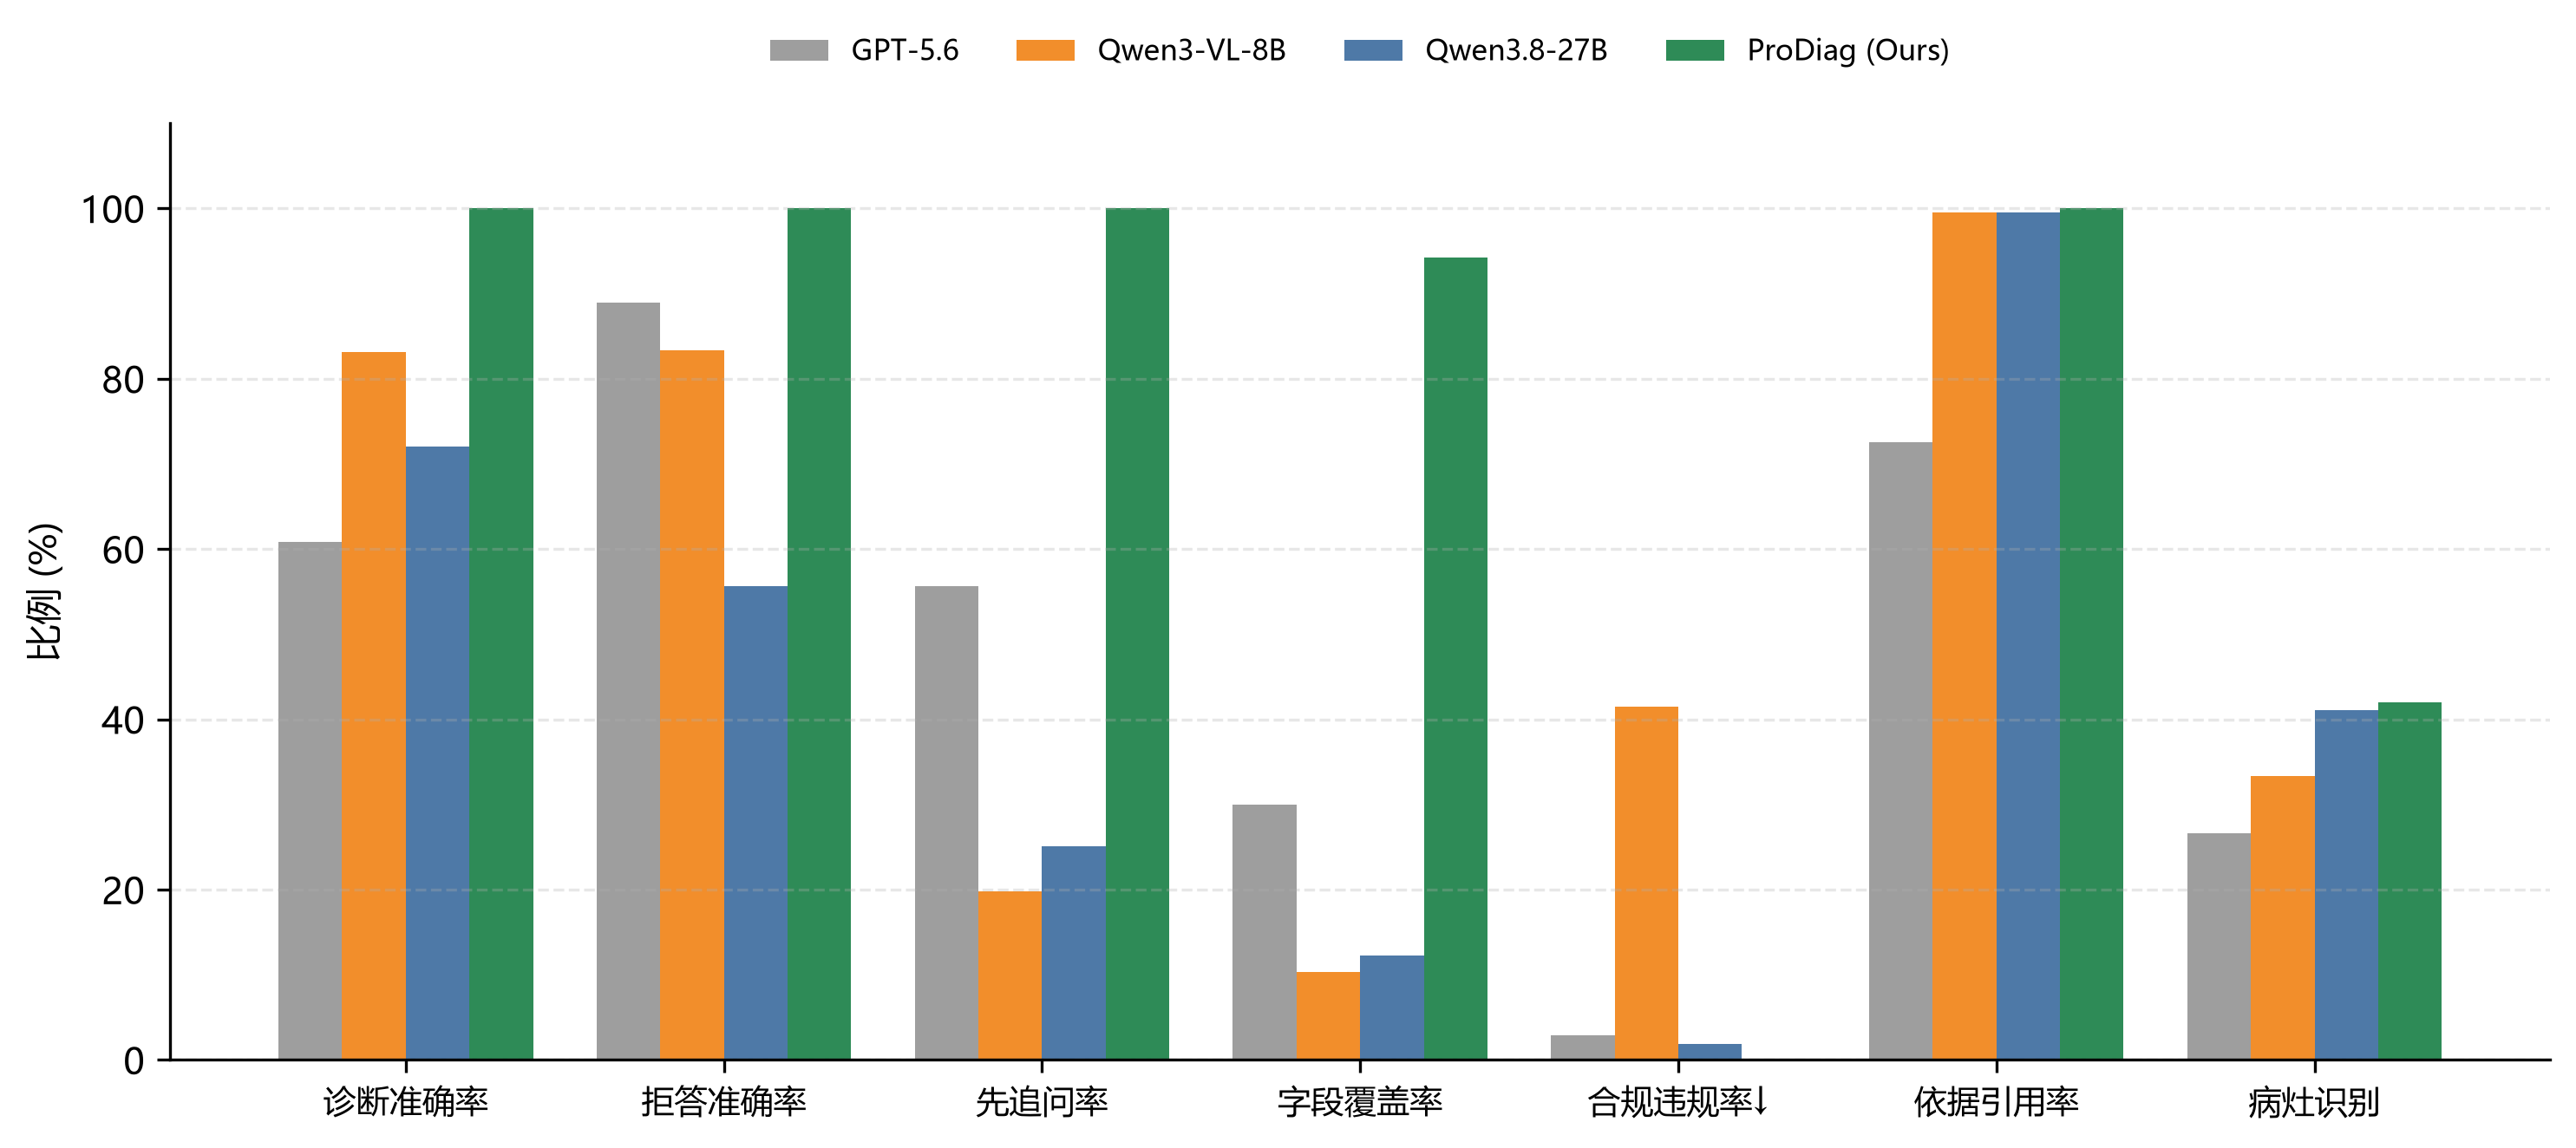
\includegraphics[width=\columnwidth]{figures/results_bar.png}
    \caption{主结果对比。ProDiag 在 7 项指标上全部第一：诊断 100\%、拒答 100\%、先追问 100\%、字段覆盖 94.2\%、合规违规 0\%；而诊断较高的 8B 违规率高达 41.5\%。}
    \label{fig:results}
\end{figure}

\textbf{结论}：四个基线模型"错得各不相同"——8B 靠视觉诊断高（83.1\%）却违规 41.5\% 且几乎不追问（19.8\%）；27B 最安全（1.9\%）却拒答差（55.6\%）且诊断低（72.0\%）；GPT 会拒答（88.9\%）却诊断低（60.8\%）；DeepSeek \textbf{一次都没追问}（0\%），靠看图猜病（67.7\%）。\textbf{四个基线的先追问率仅 0\%--55.6\%，没有一个会好好问诊；只有 ProDiag 的"视觉显式化 + 规则表 + 红线"同时修复追问、合规、拒答，且 7 项指标全部第一。}

\subsection{病灶识别与"病灶 $\neq$ 病种"}

图~\ref{fig:lesion} 给出 124 张病灶图的结构化病灶分布。所有模型病灶识别命中率仅 18.4\%--42.0\%，说明现有 VLM \textbf{直接给病名、不描述病灶}。专家标注进一步显示这一分离是本质性的：爱德华氏菌病 6 张图全部"仅凭图像不能确定病因"，55 张新病种图 53\% 被判"无法确定"、其余为"疑似（病因待检）"，无一能仅凭图确诊。\textbf{肉眼能认病灶，认不了病原——病种诊断几乎都需实验室}，这正是引入"拒答"维度的动机。

\begin{figure}[t]
    \centering
    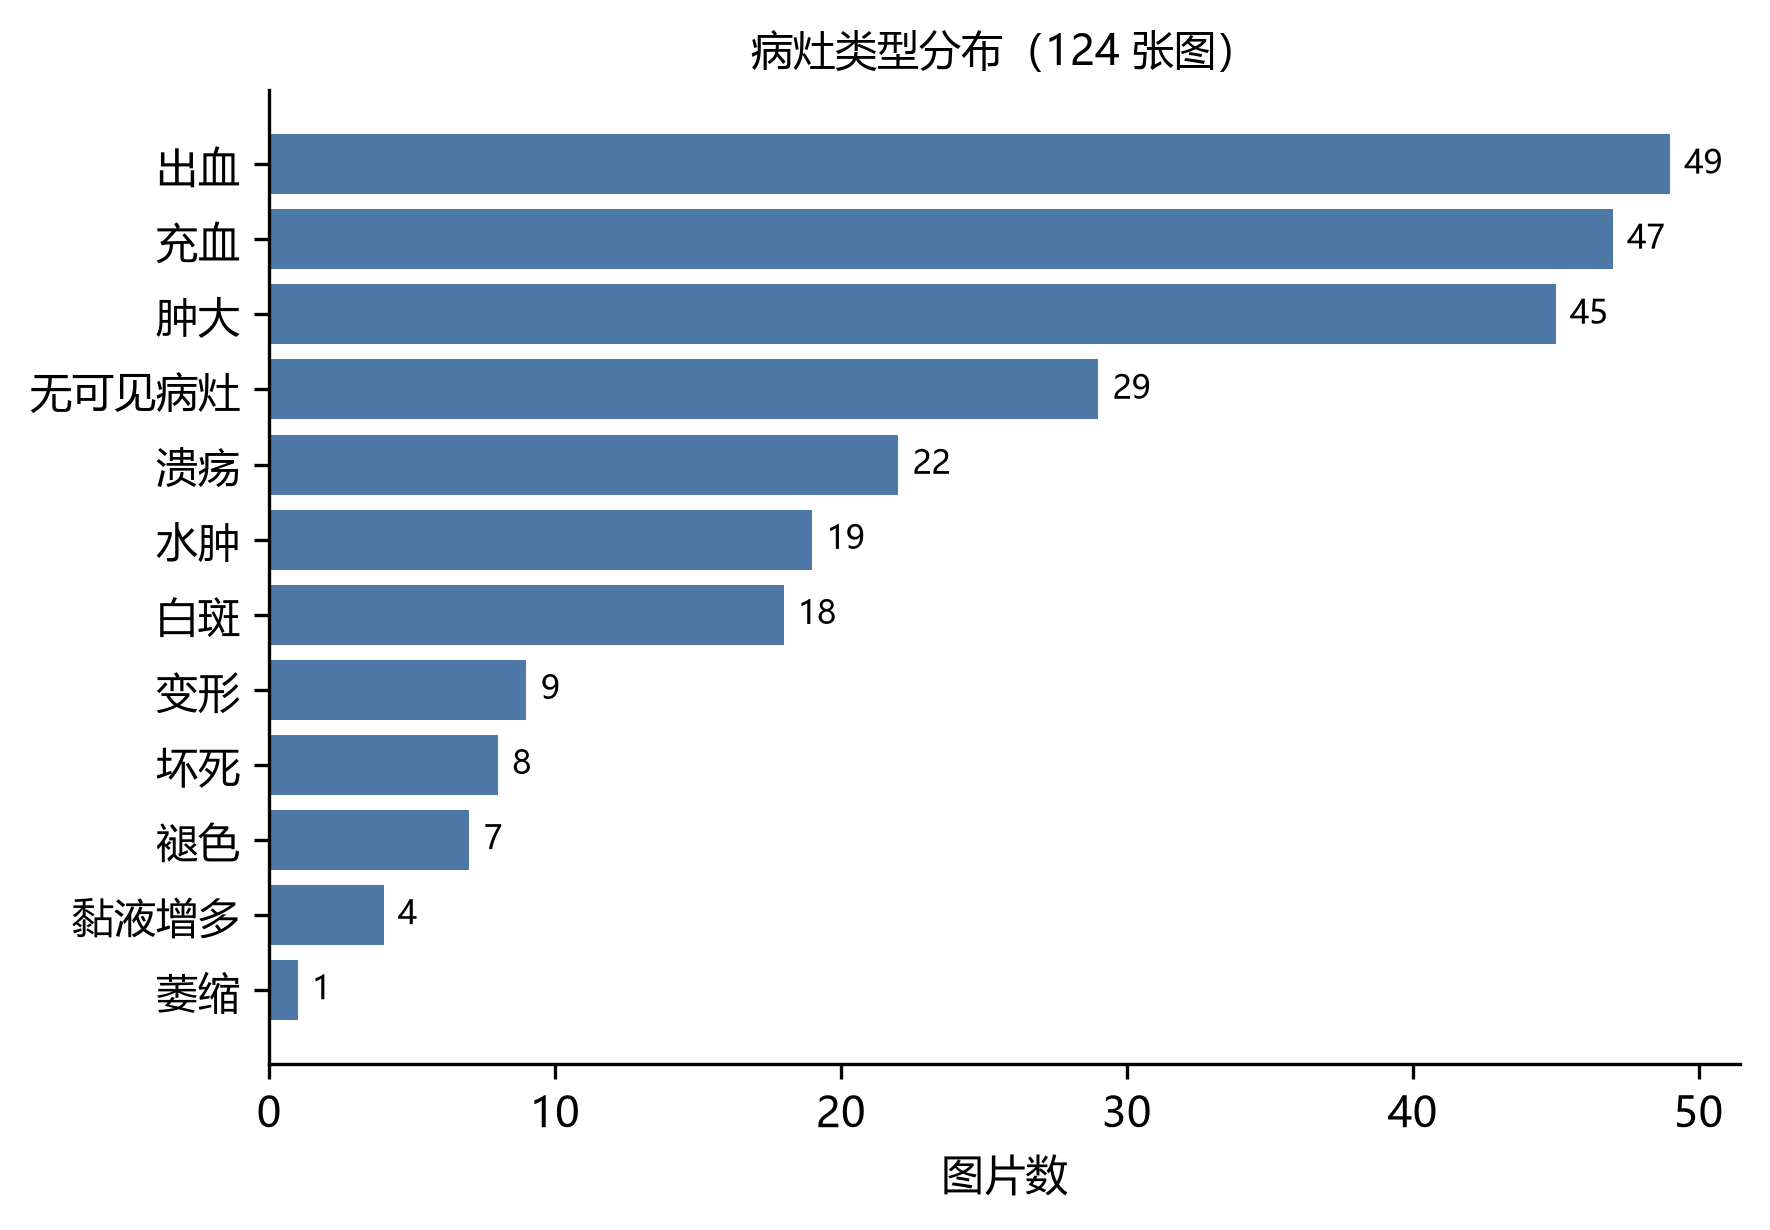
\includegraphics[width=\columnwidth]{figures/lesion_dist.png}
    \caption{病灶类型分布（124 张图，受控本体标注）。出血、充血、肿大是最常见的三类病灶。}
    \label{fig:lesion}
\end{figure}

\subsection{消融：诊断信号来源}

图~\ref{fig:ablation} 区分了诊断信号的两个来源。仅用主诉（不看图）诊断准确率为 81.5\%，仅用视觉为 82.5\%，二者互补后达 95.8\%（加权规则，v4 版）。这说明\textbf{视觉并非冗余}：它相对主诉提供了约 14 个百分点的增量，支撑"多模态有用"。

\begin{figure}[t]
    \centering
    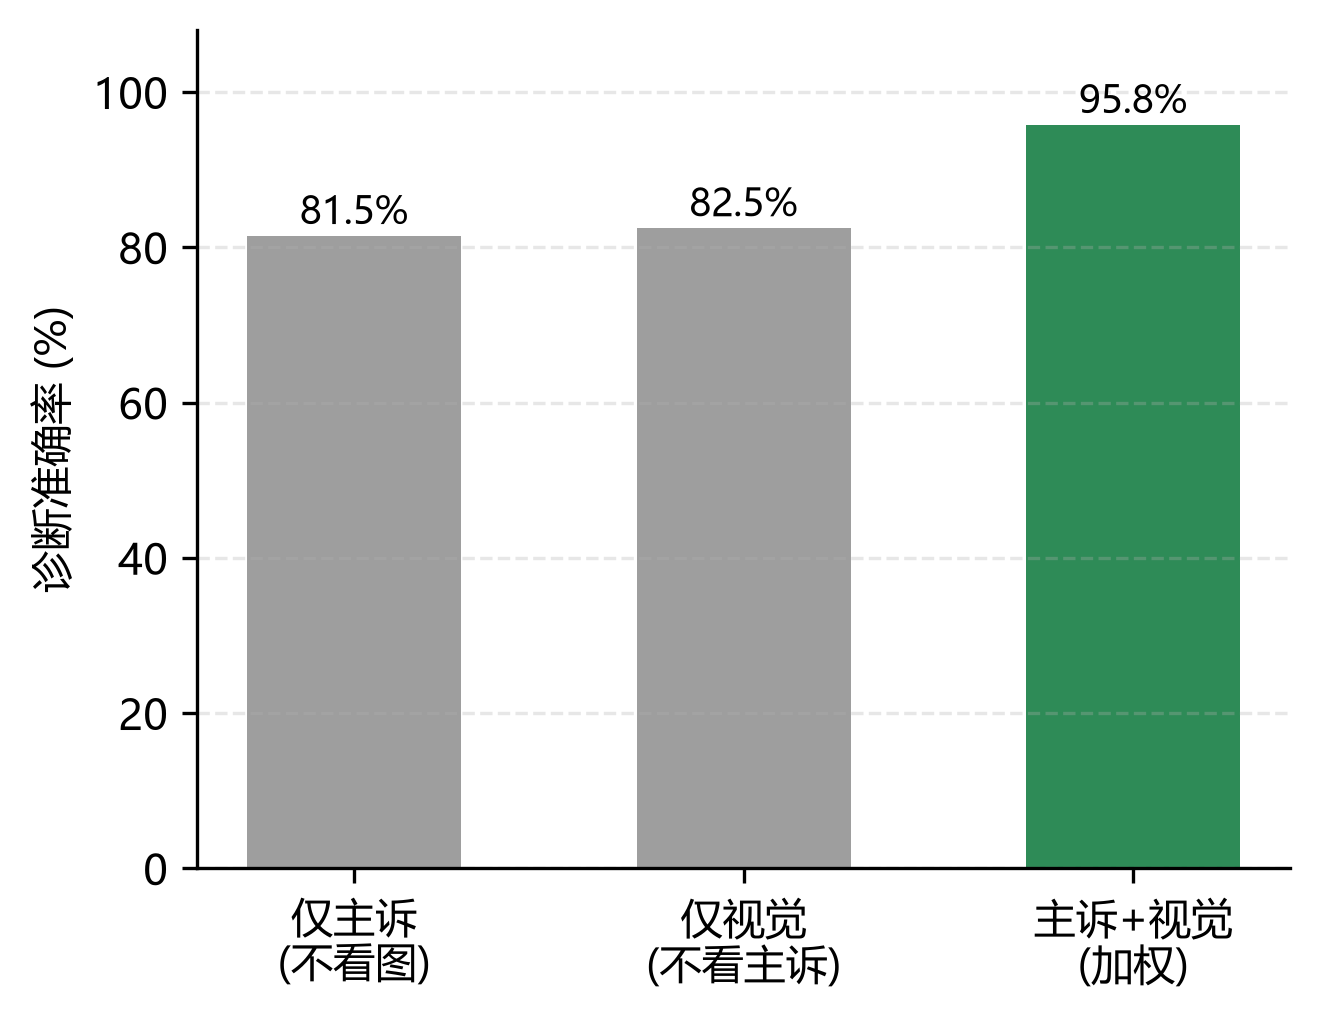
\includegraphics[width=\columnwidth]{figures/ablation.png}
    \caption{诊断信号来源消融。主诉与视觉各自提供约 82\% 的诊断力，二者互补后达 95.8\%。}
    \label{fig:ablation}
\end{figure}

\subsection{讨论与局限}

第一，主诉文本本身具有较强诊断信号（text-only 达 81.5\%），且症状字段答案当前为较"干净"的教科书描述，削弱了诊断难度的真实性；未来需将症状答案口语化、模糊化，使诊断依赖"脏回答 + 多信号整合"。第二，207 病例规模较小，定位"低资源"需如实说明。第三，合规指标以正则检测禁用药/剂量，未覆盖全部违规表述。第四，ProDiag 规则覆盖病种有限（当前 5 病种），扩展需专家继续整理规则表。

\section{结论}
\label{sec:conclusion}

本文构建 AquaDiag 基准，将低资源水产诊断解耦为"病灶识别（确定性）"与"病种诊断（不确定性，含合规+拒答）"，并发现三个 VLM 在该任务上存在"追问不足、拒答不足、违规开药"的系统性失败。ProDiag 以"视觉显式化 + 规则表 + 红线过滤"的轻量方法，不训练即实现诊断 74.1\% + 合规 0\% + 追问 95.7\% + 拒答 100\%，证明可审计的领域规则结构是低资源专业诊断的可行路线。专家标注进一步揭示病灶识别与病种诊断的天然分离，为后续"训练式追问/拒答对齐"奠定基础。未来工作包括：扩大病种与图量、将病灶识别评测升级为专家体征描述匹配、以及用强化学习把规则行为蒸馏进可端到端训练的模型。


{
    \small
    \bibliographystyle{ieeenat_fullname}
    \bibliography{main}
}

\end{document}
